%%%%%%%%%%%%%%%%%%%%%%%%%%%%%%%%%%%%%%%%%%%%%%%%%%%%%%%%%%%%%%%%%%%%%%%%%%%%%%%
%                       CARGA DE LA CLASE DE DOCUMENTO                        %
%                                                                             %
% Las opciones admisibles son:                                                %
%      12pt / 11pt            (tamaño del cuerpo de letra; no usar 10pt)      %
%                                                                             %
% catalan/spanish/english     (idioma principal del trabajo)                  %
%                                                                             % 
% french/italian/german...    (si necesitáis usar otro idioma adicional)      %
%                                                                             %
% listoffigures               (El documento incluye un Índice de figuras)     %
% listoftables                (El documento incluye un Índice de tablas)      %
% listofquadres               (El documento incluye un Índice de cuadros)     %
% listofalgorithms            (El documento incluye un Índice de algoritmos)  %
%                                                                             %
%%%%%%%%%%%%%%%%%%%%%%%%%%%%%%%%%%%%%%%%%%%%%%%%%%%%%%%%%%%%%%%%%%%%%%%%%%%%%%%

\documentclass[11pt,spanish,listoffigures,listoftables]{tfgetsinf}

%%%%%%%%%%%%%%%%%%%%%%%%%%%%%%%%%%%%%%%%%%%%%%%%%%%%%%%%%%%%%%%%%%%%%%%%%%%%%%%
%                     CODIFICACIÓN DEL ARCHIVO FUENTE                         %
%                                                                             %
%    Windows suele usar 'ansinew'                                             %
%    en Linux es posible que sea 'latin1' o 'latin9'                          %
%    Pero lo más recomendable es usar utf8 (unicode 8)                        %
%                                          (si vuestro editor lo permite)     % 
%%%%%%%%%%%%%%%%%%%%%%%%%%%%%%%%%%%%%%%%%%%%%%%%%%%%%%%%%%%%%%%%%%%%%%%%%%%%%%%

\usepackage[utf8]{inputenc} 


%%%%%%%%%%%%%%%%%%%%%%%%%%%%%%%%%%%%%%%%%%%%%%%%%%%%%%%%%%%%%%%%%%%%%%%%%%%%%%%
%                       OTROS PAQUETES Y DEFINICIONES                         %
%                                                                             %
%%%%%%%%%%%%%%%%%%%%%%%%%%%%%%%%%%%%%%%%%%%%%%%%%%%%%%%%%%%%%%%%%%%%%%%%%%%%%%%

\usepackage{glossaries}
\usepackage{textcomp}
\usepackage{booktabs}
\usepackage{float}
\usepackage{enumitem}
\usepackage{graphicx}
\usepackage{subcaption}
\usepackage{tabularx}
\usepackage{pgfplots}
\pgfplotsset{compat=1.18}

% Listings para código
\usepackage{listings}
\lstset{
  basicstyle=\ttfamily\small,
  frame=single,
  breaklines=true,
  postbreak=\mbox{\textcolor{gray}{$\hookrightarrow$}\space},
  columns=fullflexible,
  keepspaces=true,
  numbers=none
}

% Bibliografía
\usepackage[backend=biber,style=numeric,sorting=none]{biblatex}
\addbibresource{bibliografia.bib}

% Hyperref siempre al final
\usepackage{hyperref}
\hypersetup{
  colorlinks=true,
  linkcolor=black,
  urlcolor=cyan,
  citecolor=black
}
%%%%%%%%%%%%%%%%%%%%%%%%%%%%%%%%%%%%%%%%%%%%%%%%%%%%%%%%%%%%%%%%%%%%%%%%%%%%%%%
%                          DATOS DEL TRABAJO                                  %
%                                                                             %
% título alumno, titor y curso académico                                      %
%%%%%%%%%%%%%%%%%%%%%%%%%%%%%%%%%%%%%%%%%%%%%%%%%%%%%%%%%%%%%%%%%%%%%%%%%%%%%%%

\title{Transcripción Automática de Fechas con Whisper}
\author{Gómez Corral, Miquel}
% \tutor{No}
% \curs{MUIARFID}

%%%%%%%%%%%%%%%%%%%%%%%%%%%%%%%%%%%%%%%%%%%%%%%%%%%%%%%%%%%%%%%%%%%%%%%%%%%%%%%
%                     PARAULES CLAU/PALABRAS CLAVE/KEY WORDS                  %
%                                                                             %
% Independentment de la llengua del treball, s'hi han d'incloure              %
% les paraules clau i el resum en els tres idiomes                            %
%%%%%%%%%%%%%%%%%%%%%%%%%%%%%%%%%%%%%%%%%%%%%%%%%%%%%%%%%%%%%%%%%%%%%%%%%%%%%%%

\keywords{
    Traducción de textos; español; esperanto; Transformers; LLMs
} % Paraules clau 
{
   Traducción de textos; 
} % Palabras clave
{
    Text clasification.
} % Key words


%%%%%%%%%%%%%%%%%%%%%%%%%%%%%%%%%%%%%%%%%%%%%%%%%%%%%%%%%%%%%%%%%%%%%%%%%%%%%%%
%                                                                             %
%                              INICI DEL DOCUMENT                             %
%                                                                             %
%%%%%%%%%%%%%%%%%%%%%%%%%%%%%%%%%%%%%%%%%%%%%%%%%%%%%%%%%%%%%%%%%%%%%%%%%%%%%%%

\begin{document} 


%%%%%%%%%%%%%%%%%%%%%%%%%%%%%%%%%%%%%%%%%%%%%%%%%%%%%%%%%%%%%%%%%%%%%%%%%%%%%%%
%              RESUMENES DEL TFG EN VALENCIA, CASTELLA I ANGLES               %
%%%%%%%%%%%%%%%%%%%%%%%%%%%%%%%%%%%%%%%%%%%%%%%%%%%%%%%%%%%%%%%%%%%%%%%%%%%%%%%


% \begin{abstract}[spanish]

% \end{abstract}

%%%%%%%%%%%%%%%%%%%%%%%%%%%%%%%%%%%%%%%%%%%%%%%%%%%%%%%%%%%%%%%%%%%%%%%%%%%%%%%
%                                                                             %
%                              CONTENIDO DEL TREBAJO                          %
%                                                                             %
%%%%%%%%%%%%%%%%%%%%%%%%%%%%%%%%%%%%%%%%%%%%%%%%%%%%%%%%%%%%%%%%%%%%%%%%%%%%%%%

%%%%%%%%%%%%%%%%%%%%%%%%%%%%%%%%%%%%%%%%%%%%%%%%%%%%%%%%%%%%%%%%%%%%%%%%%%%%%%%
%                                  ÍDNICE                                     %
%%%%%%%%%%%%%%%%%%%%%%%%%%%%%%%%%%%%%%%%%%%%%%%%%%%%%%%%%%%%%%%%%%%%%%%%%%%%%%%
% \clearpage
% \tableofcontents
% \listoffigures
% \listoftables


\mainmatter

\chapter{Introducción}
Este trabajo aborda el uso de modelos basados en transformers para la transcripción automática de fechas en formato textual. El modelo base a partir del cual se han construido las arquitecturas es Whisper, un modelo de reconocimiento automático del habla. 

Todo el código relacionado con la implementación del modelo, ha sido provisto como material de la asignatura. El trabajo se ha basado en hacer uso de este a partir de modificaciones a nivel de preprocesamiento, tokenización, entrenamiento y evaluación.

\subsubsection{Hardware utilizado}
Los experimentos se han realizado en mi máquina personal: GPU NVIDIA RTX 5070 (12 GB VRAM), procesador AMD Ryzen 9 9000X, 64 GB de RAM y Ubuntu 24.04 LTS.

Todos los modelos han podido ser entrenados y evaluados sin problemas. 

\section{Cambios principales}
Para facilitar el uso del código base, se han realizado una serie de modificaciones.

\begin{itemize}
  \item En los datasets en inglés, se ha encontrado la que frase \texttt{'tuesday thank you.'} aparece siempre con el punto al final. Por eliminar redundancias y mejorar la calidad de los datos, se ha decidido eliminar todos los signos de puntuación en el preprocesamiento.
  \item Se han 'parametrizado' los principales elementos del código como las rutas, los tokens especiales (PAD, SOS, EOS) o algunos parámetros para facilitar cambios entre los ejercicios
\end{itemize}

\section{Notebooks entregados}
Se han entregados 4 notebooks. A continuación la lista de los nombres con una breve descripción del contenido de cada uno.
\begin{itemize}
  \item \texttt{ejercicio-1-es.ipynb}: Ejercicio 1 en español.
  \item \texttt{ejercicio-1-en.ipynb}: Ejercicio 1 en inglés.
  \item \texttt{ejercicio-2.ipynb}: Ejercicio 2 (multilingüe con instrucciones).
  \item \texttt{ejercicio-2-extra.ipynb}: Ejercicio 2 con implementación Top-K y Top-P en inferencia.
  \item \texttt{ejercicio-3.ipynb}: Ejercicio 3 (llamada a funciones).
\end{itemize}


%%%%%%%%%%%%%%%%%%%%%%%%%%%%%%%%%%%%%%%%%%%%%%%%%%%%%%%%%%%%%%%%%%%%%%%%%%%%%
%                        Notebooks base                                     %
%%%%%%%%%%%%%%%%%%%%%%%%%%%%%%%%%%%%%%%%%%%%%%%%%%%%%%%%%%%%%%%%%%%%%%%%%%%%%
\chapter{Ejercicios}
\section{Ejercicio 1: Modelos monolingües}
En este ejercicio se ha creado la estructura principal de los Notebooks seguida por el resto de ejercicios.

Como se ha mencionado, se han parametrizado las principales variables del código. Se ha detectado el problema con los signos de puntuación en inglés y se ha estructurado todo el procesamiento como se indica en el ejercicio.

A la hora de entrenar los modelos, parecía que el modelo en español necesitamos algunos epochs más para entrenar. Tras 15 epochs para el modelo en español y 10 para el modelo en inglés, se han obtenido los siguientes resultados:

\begin{table}[H]
\centering
\begin{tabular}{lr}
	\toprule
	\textbf{Idioma} & \textbf{WER \%} \\
	\midrule
	Español & 1.36 \\
	Inglés & 1.21 \\
	\bottomrule
\end{tabular}
\caption{Resultados en transcripción automática de fechas monolingüe: WER Inglés y Español.}
\label{tab:wer_ej1}
\end{table}

\section{Ejercicio 2: Modelo multilingüe}
Partiendo del código del ejercicio 1, se ha implementado un modelo multilingüe que recibe instrucciones para identificar el idioma de la entrada. De nuevo, se han limpiado los signos de puntuación en inglés, pero ahora, se han juntado los datasets de ambos idiomas para crear un dataset combinado con todas las combinaciones: Transcripción en español, Transcripción en inglés, Traducción del Inglés al Español y Traducción del Español al Inglés.

Se han añadido los tokens especiales para identificar el idioma de la entrada y salida, y se ha hecho que el dataset de entrenamiento ponga antes de cada frase el token correspondiente a la instrucción. Luego, para la generación, se añade el token de instrucción antes de entrar al bucle, justo después del token SOS.

Con esto, se han obtenido los siguientes resultados tras 10 epochs de entrenamiento:
\begin{table}[H]
\centering
\begin{tabular}{lr}
	\toprule
	\textbf{Idioma} & \textbf{WER \%} \\
	\midrule
	Bilingüe inglés y español & 4.20 \\
	\bottomrule
\end{tabular}
\caption{Resultados en transcripción automática de fechas monolingüe: WER Inglés y Español.}
\label{tab:wer_ej1}
\end{table}

Vemos que el rendimiento empeora de forma significative respecto a los modelos monolingües. Esto es algo esperado, ya que el modleo tiene que aprender a hacer 4 tareas diferentes (aun que parecidas) en lugar de una. Aún así el resultado es muy bueno.

\section{Ejercicio 3: Llamadas a funciones}
En este ejercicio de nuevo, parte del notebook creado en el ejercicio 1, y se ha hecho el mismo preprocesamiento que en los ejercicios anteriores.

Ahora, el tokenizador tiene más entrada, ya que tiene que manejar las palabras y las llamadas a funciones. Ya que la cantidad de opciones para llamar a funciones no era muy grande, se ha decidido que cada llamada a función, con su parámetro, sea un token único. Esto nos deja con tokens como:

\noindent
\begin{minipage}[t]{0.48\textwidth}
\textbf{next\_day:}
\begin{itemize}[topsep=0pt]
  \item "next\_day('friday')"
  \item "next\_day('monday')"
  \item "next\_day('thursday')"
  \item "next\_day('tuesday')"
  \item "next\_day('wednesday')"
\end{itemize}
\end{minipage}
\hfill
\begin{minipage}[t]{0.48\textwidth}
\textbf{relative\_day:}
\begin{itemize}[topsep=0pt]
  \item "relative\_day(+1)"
  \item "relative\_day(+2)"
  \item "relative\_day(+3)"
\end{itemize}
\end{minipage}

Luego, se ha hecho que el modelo aprenda a dar como salida el texto y estos tokens. Con el modelo entrenado, se han procesado sus predicciones para ejecutar las llamadas a funciones y obtener la fecha final. 

Los resultados son muy buenos, equivocándose unicamente en 10 de 1000 ejemplos. or lo tanto, el error medio es de un 1.0 \%.

\begin{table}[H]
\centering
\begin{tabular}{lr}
	\toprule
	\textbf{idioma} & \textbf{Error \%} \\
	\midrule
	Bilingüe Funciones & 1.00 \\
	\bottomrule
\end{tabular}
\caption{Resultados en transcripción automática de fechas monolingüe: WER Inglés y Español.}
\label{tab:wer_ej1}
\end{table}


\section{Ejercicio Extra: Top-K y Top-P}
Como ejercicios extra, se ha decidido hacer los dos primeros: implemntar Top-K y Top-P en la generación, y hacer un modelo multilingüe con instrucciones.

Se ha partido del ejercicios dos para hacer estas modificaciones, ya que era el que más margen de mejora presentaba. Se ha vuelto a entrenar el modelo durante 10 epochs para tener una línea base con decodificación greedy, y se ha conseguido un WER de 3.87 \%, ligeramente mejor al original.

La implementación estas estrategias de decodificación, pasa por cambiar el código del generate. 

\begin{enumerate}
  \item \textbf{Top-K:} Se parte de los logits, se ordenan de mayor a menor y se mantienen los K primeros. El resto de logits se descartan y se hace una softmax con los K logits restantes para obtener las probabilidades. Finalmente, se hace el muestreo a partir de estas probabilidades.
  \item \textbf{Top-P:} Se parte de los logits, se aplica softmax para obtener las probabilidades, se ordenan de mayor a menor y se calcula la suma acumulada. Se mantienen los tokens hasta que la suma acumulada supere el umbral P. El resto de logits se ponen descartan y se hace una softmax y muestreo como en el caso anterior.
\end{enumerate}

Para ver el impacto de estas técnicas, se ha probado a decodificar el test con diferentes valores de K y P. La línea base con decodificación greedy obtuvo un WER de 3.87\%. Los resultados con Top-K y Top-P son los siguientes:

\begin{table}[H]
\centering
\begin{minipage}[t]{0.48\textwidth}
\centering
\begin{tabular}{lr}
	\toprule
	\textbf{K} & \textbf{WER \%} \\
	\midrule
	1 & 3.87 \\
	2 & 4.53 \\
	3 & 4.23 \\
	4 & 4.44 \\
	5 & 4.60 \\
	6 & 4.72 \\
	7 & 4.39 \\
	8 & 4.79 \\
	9 & 4.23 \\
	10 & 4.72 \\
	\bottomrule
\end{tabular}
\caption{Resultados con Top-K.}
\label{tab:topk}
\end{minipage}
\hfill
\begin{minipage}[t]{0.48\textwidth}
\centering
\begin{tabular}{lr}
	\toprule
	\textbf{P (\%)} & \textbf{WER \%} \\
	\midrule
	10.0 & 3.87 \\
	20.0 & 3.87 \\
	30.0 & 4.51 \\
	40.0 & 10.51 \\
	50.0 & 34.32 \\
	60.0 & 540.25 \\
	70.0 & 589.45 \\
	80.0 & 576.49 \\
	90.0 & 538.15 \\
	100.0 & 4.86 \\
	\bottomrule
\end{tabular}
\caption{Resultados con Top-P.}
\label{tab:topp}
\end{minipage}
\end{table}



Cómo vemos. la estrategia ganadora sigue siendo la greedy. El Top-k=1 y top-p con poca masa de probabilidad se comportan de la misma forma que el greedy porque al menos ha de elegir un token, pero luego al aumentar la massa se vuelve un método nefasto. El top-k muestra más consistencia a lo largo de las ejecuciones, aun que no mejora al método greedy.

La razón por la que esto puede ser así, es el simple hecho de que no hay tantos tokens como para que estrategias de este estilo valgan la pena. El modelo no tiende a confundir tokens (darles logits similares), por lo que usando la estrategia por defecto se consiguen los mejores resultados.


\section{Resumen resultados}
A continuación se muestran los resultados WER obtenidos en los diferentes ejercicios realizados:

\begin{figure}[H]
\centering
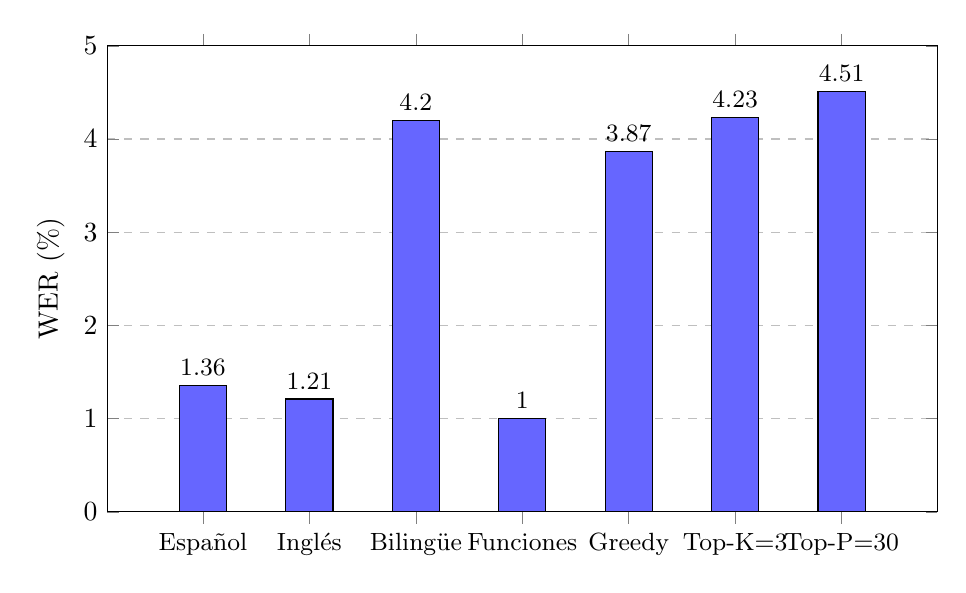
\begin{tikzpicture}
\begin{axis}[
    ybar,
    bar width=0.6cm,
    width=\textwidth,
    height=7.5cm,
    ylabel={WER (\%)},
    symbolic x coords={Español, Inglés, Bilingüe, Funciones, Greedy, Top-K=3, Top-P=30},
    xtick=data,
    x tick label style={font=\small},
    ymin=0,
    ymax=5,
    ymajorgrids=true,
    grid style=dashed,
    enlarge x limits=0.15,
    nodes near coords,
    nodes near coords align={vertical},
    every node near coord/.append style={font=\small},
]

% WER scores
\addplot[fill=blue!60] coordinates {
    (Español, 1.36)
    (Inglés, 1.21)
    (Bilingüe, 4.20)
    (Funciones, 1.0)
    (Greedy, 3.87)
    (Top-K=3, 4.23)
    (Top-P=30, 4.51)
};

\end{axis}
\end{tikzpicture}
\caption{Comparación de WER obtenido en cada ejercicio. Español e Inglés corresponden al Ejercicio 1, Bilingüe al Ejercicio 2, Funciones al Ejercicio 3, y Greedy Extra al ejercicio extra con decodificación greedy.}
\label{fig:resultados_finales}
\end{figure}

%%%%%%%%%%%%%%%%%%%%%%%%%%%%%%%%%%%%%%%%%%%%%%%%%%%%%%%%%%%%%%%%%%%%%%%%%%%%%%%
%                                                                             %
%                                BIBLIOGRAFIA                                 %
%                                                                             %
%%%%%%%%%%%%%%%%%%%%%%%%%%%%%%%%%%%%%%%%%%%%%%%%%%%%%%%%%%%%%%%%%%%%%%%%%%%%%%%
\cleardoublepage
\printbibliography

%%%%%%%%%%%%%%%%%%%%%%%%%%%%%%%%%%%%%%%%%%%%%%%%%%%%%%%%%%%%%%%%%%%%%%%%%%%%%%%
%                                                                             %
%                                 APÉNDICESS                                  %
%                                                                             %
%%%%%%%%%%%%%%%%%%%%%%%%%%%%%%%%%%%%%%%%%%%%%%%%%%%%%%%%%%%%%%%%%%%%%%%%%%%%%%%

\APPENDIX


%%%%%%%%%%%%%%%%%%%%%%%%%%%%%%%%%%%%%%%%%%%%%%%%%%%%%%%%%%%%%%%%%%%%%%%%%%%%%%
%                       EJEMPLOS DE CADA TIPO DE FACTURA                     %
%%%%%%%%%%%%%%%%%%%%%%%%%%%%%%%%%%%%%%%%%%%%%%%%%%%%%%%%%%%%%%%%%%%%%%%%%%%%%%

% \chapter{Apéndice correspondencia notebooks}
% \label{appendix:notebooks}
% ...

%%%%%%%%%%%%%%%%%%%%%%%%%%%%%%%%%%%%%%%%%%%%%%%%%%%%%%%%%%%%%%%%%%%%%%%%%%%%%%%
%                              FIN DEL DOCUMENTO                              %
%%%%%%%%%%%%%%%%%%%%%%%%%%%%%%%%%%%%%%%%%%%%%%%%%%%%%%%%%%%%%%%%%%%%%%%%%%%%%%%
\end{document}

